\documentclass[12pt, a4paper]{article}
\usepackage[utf8]{inputenc}
\usepackage{geometry}
\geometry{top=2.5cm, bottom=2.5cm, left=2.5cm, right=2.5cm}
\usepackage{amsmath, amssymb, amsthm}
\usepackage{graphicx}
\usepackage{enumitem}
\usepackage{hyperref}
\usepackage{tcolorbox}
\tcbuselibrary{skins, breakable}
\usepackage{tikz}
\usetikzlibrary{shapes, arrows, positioning, fit, calc, automata, arrows.meta}
\usepackage{float}
\usepackage{titlesec}
\usepackage{framed}

% Use a simpler, cleaner box style
\tcbset{
    enhanced,
    colback=white,
    colframe=black!75!white,
    boxrule=0.5pt,
    arc=0mm,
    top=2mm, bottom=2mm, left=2mm, right=2mm,
    title style={fill=none, coltext=black, font=\bfseries\large},
    detach title,
    before upper={\tcbtitle\par\vspace{2mm}}
}

% Problem Box: Light Blue background
\newtcolorbox{problembox}[2][]{
    title={Problem #2},
    colback=blue!5!white,
    colframe=blue!50!black,
    coltitle=black,
    colbacktitle=blue!10!white,
    fonttitle=\bfseries\large,
    attach boxed title to top left={xshift=5mm, yshift*=-3mm},
    boxed title style={colframe=blue!50!black, size=small},
    drop shadow=black!10!white,
    #1
}

% Guide Box: Light Orange/Yellow background
\newtcolorbox{guidebox}[1][]{
    title={Guide / Hint},
    colback=orange!5!white,
    colframe=orange!80!black,
    coltitle=white,
    fonttitle=\bfseries\normalsize,
    fontupper=\itshape,
    #1
}

% Solution Box: Light Green background
\newtcolorbox{solutionbox}[1][]{
    title={Detailed Step-by-Step Solution},
    colback=green!5!white,
    colframe=green!40!black,
    coltitle=white,
    fonttitle=\bfseries\normalsize,
    #1
}

\title{\textbf{\Huge Deep Reinforcement Learning Practice Guide}\\
\large A Collection of 48 Exam-Style Numerical Problems with Detailed Solutions}
\author{Comprehensive Preparation Material}
\date{\today}

\begin{document}

\maketitle
\tableofcontents
\newpage

\section*{Introduction}
This practice guide contains 48 distinct numerical problems designed to test your understanding of Reinforcement Learning concepts, from basic Multi-Armed Bandits to advanced Deep RL architectures like AlphaGo.

Each problem is structured with:
\begin{itemize}
    \item \textbf{Problem Statement}: A clear, exam-style question.
    \item \textbf{Guide / Hint}: Initial steps or formulas to help you get started.
    \item \textbf{Step-by-Step Solution}: A detailed walkthrough of the calculation, showing:
        \begin{itemize}
            \item \textbf{Given}: Variables extracted from the problem.
            \item \textbf{Formula}: The generic equation used.
            \item \textbf{Explanation}: Why this formula is relevant.
            \item \textbf{Calculation}: Intermediate arithmetic steps.
            \item \textbf{Final Answer}: The result interpreted.
        \end{itemize}
\end{itemize}

\section*{How to Use This Guide}
To maximize your learning:
1.  **Attempt First**: Read the problem statement and try to solve it on paper before looking at the solution.
2.  **Identify Variables**: Extract key variables ($S, A, R, \gamma, \alpha, \epsilon$) from the scenario text.
3.  **Draw Diagrams**: For MDP and GridWorld problems, sketch the states and transitions.
4.  **Check Formulas**: Refer to the "Guide / Hint" box if you are stuck on which formula to apply.
5.  **Verify Calculation**: Compare your final numerical answer with the provided solution.

\newpage

% ----------------------------------------------------------------------
% TOPIC 1: RL BASICS & MDPS
% ----------------------------------------------------------------------
\section{Topic 1: RL Basics \& MDPs}
\textit{Topics Covered: Multi-Armed Bandits, Exploration vs Exploitation, Markov Decision Processes, Bellman Equations, Value Iteration, Policy Iteration.}

% Problem 1.1
\begin{problembox}{1.1: Epsilon-Greedy Portfolio Management}
A high-frequency trading bot manages a portfolio with 4 crypto assets $\{a_1, a_2, a_3, a_4\}$. It uses an $\epsilon$-greedy policy with $\epsilon = 0.2$ to select which asset to buy. Currently, the estimated returns (Q-values) are $Q(a_1)=1.5, Q(a_2)=2.2, Q(a_3)=0.8, Q(a_4)=2.2$.
Calculate the probability of selecting each asset $a_i$ under this policy. Note that there is a tie for the best asset.
\end{problembox}

\begin{guidebox}
Remember that the probability of selecting a greedy action is $1 - \epsilon + \frac{\epsilon}{|A|}$ (split among ties) and a non-greedy action is $\frac{\epsilon}{|A|}$.
\end{guidebox}

\begin{solutionbox}
\begin{center}
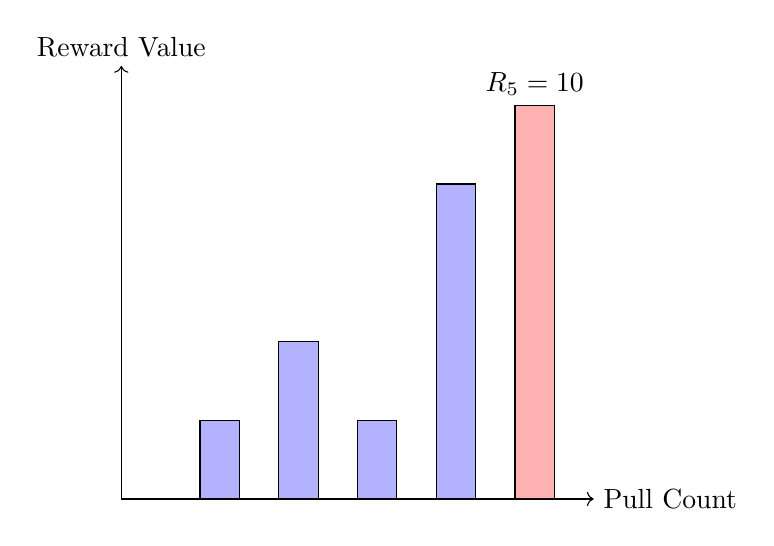
\begin{tikzpicture}[x=1cm, y=0.5cm]
    \draw[->] (0,0) -- (6,0) node[right] {Pull Count};
    \draw[->] (0,0) -- (0,11) node[above] {Reward Value};
    \foreach \x/\y in {1/2, 2/4, 3/2, 4/8}
        \draw[fill=blue!30] (\x,0) rectangle (\x+0.5,\y);
    \node[above] at (5.25, 10) {$R_5=10$};
    \draw[fill=red!30] (5,0) rectangle (5.5, 10);
\end{tikzpicture}
\end{center}

\textbf{1. Given:}
\begin{itemize}
    \item Actions (Assets): $A = \{a_1, a_2, a_3, a_4\}$
    \item Number of actions: $|A| = 4$
    \item Exploration rate: $\epsilon = 0.2$
    \item Q-values: $Q(a_1)=1.5, Q(a_2)=2.2, Q(a_3)=0.8, Q(a_4)=2.2$
\end{itemize}

\textbf{2. Identify Greedy Actions:}
The greedy actions are those with the maximum Q-value.
$$ \max_a Q(a) = 2.2 $$
The actions with this value are $a_2$ and $a_4$.
Let $A^*$ be the set of greedy actions. $|A^*| = 2$.

\textbf{3. Formulas:}
The policy probability $\pi(a|s)$ depends on whether action $a$ is greedy or not.
\begin{itemize}
    \item For a non-greedy action $a \notin A^*$:
      $$ \pi(a) = \frac{\epsilon}{|A|} $$
    \item For a greedy action $a \in A^*$:
      $$ \pi(a) = \frac{\epsilon}{|A|} + \frac{1 - \epsilon}{|A^*|} $$
      (The exploration probability is shared equally among all actions, and the exploitation probability $1-\epsilon$ is shared among the greedy actions).
\end{itemize}

\textbf{4. Explanation:}
Since we follow an $\epsilon$-greedy strategy, we explore with probability $\epsilon$ (choosing randomly among all 4 actions) and exploit with probability $1-\epsilon$ (choosing uniformly among the best actions).

\textbf{5. Calculation:}
\textit{Exploration Component per Action:}
$$ \frac{\epsilon}{|A|} = \frac{0.2}{4} = 0.05 $$

\textit{Exploitation Component per Greedy Action:}
$$ \frac{1 - \epsilon}{|A^*|} = \frac{1 - 0.2}{2} = \frac{0.8}{2} = 0.4 $$

\textit{Total Probabilities:}
\begin{itemize}
    \item For Non-Greedy Actions ($a_1, a_3$):
      $$ \pi(a_1) = \pi(a_3) = 0.05 $$
    \item For Greedy Actions ($a_2, a_4$):
      $$ \pi(a_2) = \pi(a_4) = 0.05 + 0.4 = 0.45 $$
\end{itemize}

\textbf{6. Final Answer:}
- $P(a_1) = 0.05$
- $P(a_2) = 0.45$
- $P(a_3) = 0.05$
- $P(a_4) = 0.45$

(Check: $0.05 + 0.45 + 0.05 + 0.45 = 1.0$).
\end{solutionbox}
\newpage

% Problem 1.2
\begin{problembox}{1.2: Sample Average Update}
A bandit algorithm has pulled arm A 4 times with rewards: $\{2, 4, 2, 8\}$.
(a) Calculate the current estimated value $Q_4(A)$.
(b) The arm is pulled a 5th time and yields a reward of $R_5 = 10$. Update the Q-value using the incremental update rule $Q_{n+1} = Q_n + \frac{1}{n}(R_n - Q_n)$.
\end{problembox}

\begin{guidebox}
Use the definition $Q_n = \frac{R_1 + \dots + R_{n-1}}{n-1}$. For part (b), apply the formula with $n=5$ (since it's the 5th update, using the count *including* the new reward). Note: standard notation is $Q_{k+1}$ after $k$ selections.
\end{guidebox}

\begin{solutionbox}
\begin{center}
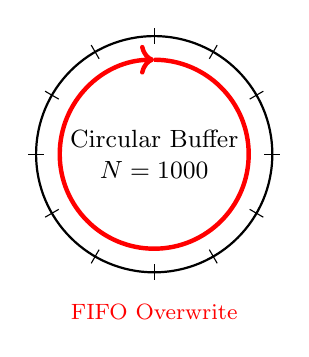
\begin{tikzpicture}
  \draw[thick] (0,0) circle (1.5cm);
  \foreach \angle in {0, 30, ..., 330}
    \draw (\angle:1.4cm) -- (\angle:1.6cm);
  \draw[->, ultra thick, red] (90:1.2cm) arc (90:-270:1.2cm);
  \node[align=center, font=\small] at (0,0) {Circular Buffer\\$N=1000$};
  \node[red, font=\footnotesize] at (0, -2) {FIFO Overwrite};
\end{tikzpicture}
\end{center}

\textbf{1. Given:}
\begin{itemize}
    \item History of rewards: $R_1=2, R_2=4, R_3=2, R_4=8$.
    \item Number of previous pulls: $n_{old} = 4$.
    \item New reward: $R_5 = 10$.
\end{itemize}

\textbf{Part (a): Current Estimate $Q_4(A)$}
\textit{Formula:} Simple average: $Q_n = \frac{\sum R_i}{n}$.
\textit{Calculation:}
Sum = $2 + 4 + 2 + 8 = 16$.
$$ Q_4(A) = \frac{16}{4} = 4.0 $$

\textbf{Part (b): Incremental Update}
\textit{Formula:}
$$ Q_{new} = Q_{old} + \frac{1}{n_{new}} (R_{new} - Q_{old}) $$
Where $n_{new} = 5$ is the total count after the update.

\textit{Substitution:}
\begin{itemize}
    \item $Q_{old} = 4.0$
    \item $n_{new} = 5$
    \item $R_{new} = 10$
\end{itemize}
$$ Q_5(A) = 4.0 + \frac{1}{5} (10 - 4.0) $$

\textit{Calculation:}
$$ Q_5(A) = 4.0 + 0.2 (6) $$
$$ Q_5(A) = 4.0 + 1.2 $$
$$ Q_5(A) = 5.2 $$

\textbf{Final Answer:}
(a) $Q_4(A) = 4.0$
(b) $Q_5(A) = 5.2$
\end{solutionbox}
\newpage

% Problem 1.3
\begin{problembox}{1.3: UCB1 Action Selection}
You have a 3-armed bandit. At time step $t=100$, the counts and estimated values are:
- Arm 1: $N_1=20, Q_1=0.8$
- Arm 2: $N_2=70, Q_2=1.0$
- Arm 3: $N_3=10, Q_3=1.2$
Using the UCB1 formula with exploration parameter $c=2$, which arm should be selected next? (Use $\ln t$ for the natural logarithm).
\end{problembox}

\begin{guidebox}
Calculate $UCB = Q_a + c \sqrt{\frac{\ln t}{N_a}}$ for each arm.
\end{guidebox}

\begin{solutionbox}
\begin{center}
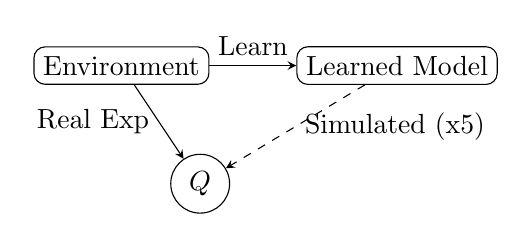
\begin{tikzpicture}[node distance=1.5cm, auto, >=stealth]
  \node[draw, rounded corners] (env) {Environment};
  \node[draw, rounded corners, right of=env, xshift=2cm] (model) {Learned Model};
  \node[draw, circle, below of=env, xshift=1cm] (q) {$Q$};

  \draw[->] (env) -- node[left] {Real Exp} (q);
  \draw[->, dashed] (model) -- node[right] {Simulated (x5)} (q);
  \draw[->] (env) -- node[above] {Learn} (model);
\end{tikzpicture}
\end{center}

\textbf{1. Given:}
\begin{itemize}
    \item Time step $t=100$.
    \item Exploration constant $c=2$.
    \item Arm 1: $N_1=20, Q_1=0.8$.
    \item Arm 2: $N_2=70, Q_2=1.0$.
    \item Arm 3: $N_3=10, Q_3=1.2$.
\end{itemize}

\textbf{2. Formula:}
The Upper Confidence Bound (UCB) value for an action $a$ is:
$$ U_t(a) = Q_t(a) + c \sqrt{\frac{\ln t}{N_t(a)}} $$
We select $A_t = \arg\max_a U_t(a)$.

\textbf{3. Explanation:}
UCB balances exploitation ($Q_t(a)$) with exploration (the square root term). Actions with fewer visits ($N_t(a)$) have higher uncertainty and thus a higher bonus.

\textbf{4. Calculation:}
First, calculate $\ln t$:
$$ \ln(100) \approx 4.605 $$

\textit{Arm 1:}
$$ U_1 = 0.8 + 2 \sqrt{\frac{4.605}{20}} $$
$$ U_1 = 0.8 + 2 \sqrt{0.23025} $$
$$ U_1 \approx 0.8 + 2(0.48) = 0.8 + 0.96 = 1.76 $$

\textit{Arm 2:}
$$ U_2 = 1.0 + 2 \sqrt{\frac{4.605}{70}} $$
$$ U_2 = 1.0 + 2 \sqrt{0.0658} $$
$$ U_2 \approx 1.0 + 2(0.256) = 1.0 + 0.51 = 1.51 $$

\textit{Arm 3:}
$$ U_3 = 1.2 + 2 \sqrt{\frac{4.605}{10}} $$
$$ U_3 = 1.2 + 2 \sqrt{0.4605} $$
$$ U_3 \approx 1.2 + 2(0.678) = 1.2 + 1.35 = 2.55 $$

\textbf{5. Comparison:}
$U_1=1.76, U_2=1.51, U_3=2.55$.
The maximum value is $2.55$ (Arm 3).

\textbf{Final Answer:}
Select \textbf{Arm 3}.
\end{solutionbox}
\newpage

% Problem 1.4
\begin{problembox}{1.4: Autonomous Vehicle Navigation}
A self-driving car navigates a complex intersection. An episode yields the following reward sequence:
- $t=1$: Correct turn ($R_1=2$)
- $t=2$: Wait for light ($R_2=0$)
- $t=3$: Avoid pedestrian ($R_3=5$)
- $t=4$: Reach destination ($R_4=10$, Terminal)
Calculate the discounted return $G_0$ (from time $t=0$) with a discount factor $\gamma = 0.9$.
\end{problembox}

\begin{guidebox}
$G_t = R_{t+1} + \gamma R_{t+2} + \gamma^2 R_{t+3} + \dots$
\end{guidebox}

\begin{solutionbox}
\begin{center}
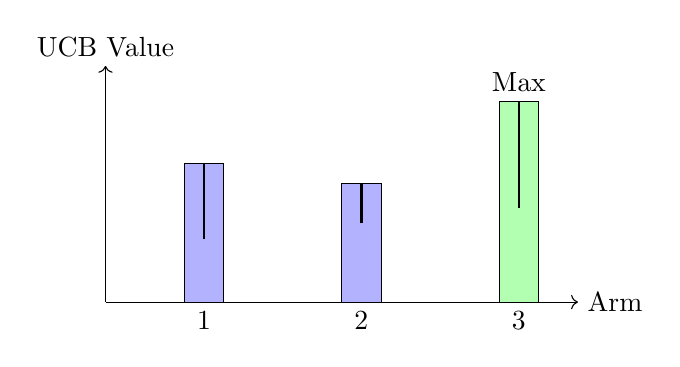
\begin{tikzpicture}
    % Axis
    \draw[->] (0,0) -- (6,0) node[right] {Arm};
    \draw[->] (0,0) -- (0,3) node[above] {UCB Value};

    % Bars
    \draw[fill=blue!30] (1,0) rectangle (1.5, 1.76) node[midway, black] {};
    \node[below] at (1.25, 0) {1};

    \draw[fill=blue!30] (3,0) rectangle (3.5, 1.51) node[midway, black] {};
    \node[below] at (3.25, 0) {2};

    \draw[fill=green!30] (5,0) rectangle (5.5, 2.55) node[midway, black] {};
    \node[below] at (5.25, 0) {3};

    % Error bars (symbolic of exploration)
    \draw[thick] (1.25, 0.8) -- (1.25, 1.76);
    \draw[thick] (3.25, 1.0) -- (3.25, 1.51);
    \draw[thick] (5.25, 1.2) -- (5.25, 2.55);

    \node at (5.25, 2.8) {Max};
\end{tikzpicture}
\end{center}

\textbf{1. Given:}
\begin{itemize}
    \item Rewards: $R_1=2, R_2=0, R_3=5, R_4=10$.
    \item Discount factor: $\gamma=0.9$.
    \item Start time: $t=0$.
\end{itemize}

\textbf{2. Formula:}
The discounted return $G_t$ is the sum of future discounted rewards:
$$ G_t = \sum_{k=0}^{\infty} \gamma^k R_{t+k+1} $$
For $t=0$:
$$ G_0 = R_1 + \gamma R_2 + \gamma^2 R_3 + \gamma^3 R_4 $$

\textbf{3. Explanation:}
Future rewards are worth less than immediate rewards by a factor of $\gamma$ per time step. We sum them up to find the total value of the trajectory.

\textbf{4. Calculation:}
Substitute values:
$$ G_0 = 2 + (0.9)(0) + (0.9)^2(5) + (0.9)^3(10) $$

Compute powers:
- $\gamma^1 = 0.9$
- $\gamma^2 = 0.81$
- $\gamma^3 = 0.729$

Calculate terms:
- Term 1: $2$
- Term 2: $0$
- Term 3: $0.81 \times 5 = 4.05$
- Term 4: $0.729 \times 10 = 7.29$

Sum:
$$ G_0 = 2 + 0 + 4.05 + 7.29 $$
$$ G_0 = 13.34 $$

\textbf{Final Answer:}
$G_0 = 13.34$
\end{solutionbox}
\newpage

% Problem 1.5
\begin{problembox}{1.5: Bellman Expectation for $V_\pi$}
Consider a state $s$ with two actions $a_1$ and $a_2$.
- Under policy $\pi$: $\pi(a_1|s) = 0.6, \pi(a_2|s) = 0.4$.
- Action $a_1$: transitions to $s'$ with probability 1.0, reward $R=2$. $V_\pi(s') = 10$.
- Action $a_2$: transitions to $s''$ with probability 1.0, reward $R=-1$. $V_\pi(s'') = 5$.
Calculate $V_\pi(s)$ assuming $\gamma=0.5$.
\end{problembox}

\begin{guidebox}
$V_\pi(s) = \sum_a \pi(a|s) \sum_{s',r} p(s',r|s,a) [r + \gamma V_\pi(s')]$.
\end{guidebox}

\begin{solutionbox}
\begin{center}
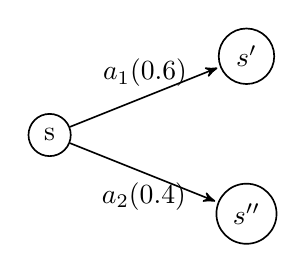
\begin{tikzpicture}[->, >=stealth', shorten >=1pt, auto, node distance=2.5cm, semithick]
  \node[circle, draw] (s) {s};
  \node[circle, draw, right of=s, yshift=1cm] (s1) {$s'$};
  \node[circle, draw, right of=s, yshift=-1cm] (s2) {$s''$};

  \path (s) edge node [above] {$a_1 (0.6)$} (s1)
        (s) edge node [below] {$a_2 (0.4)$} (s2);
\end{tikzpicture}
\end{center}

\textbf{1. Given:}
\begin{itemize}
    \item Policy: $\pi(a_1|s)=0.6, \pi(a_2|s)=0.4$.
    \item Discount: $\gamma=0.5$.
    \item Path 1: $R=2, V(s')=10$.
    \item Path 2: $R=-1, V(s'')=5$.
\end{itemize}

\textbf{2. Formula:}
Bellman Expectation Equation:
$$ V_\pi(s) = \sum_{a} \pi(a|s) \left[ R(s,a) + \gamma \sum_{s'} P(s'|s,a) V_\pi(s') \right] $$
Since transitions are deterministic ($P=1$), this simplifies to:
$$ V_\pi(s) = \pi(a_1|s)[R_1 + \gamma V(s')] + \pi(a_2|s)[R_2 + \gamma V(s'')] $$

\textbf{3. Explanation:}
The value of a state is the weighted average of the values of taking each action. The value of an action is the immediate reward plus the discounted value of the next state.

\textbf{4. Calculation:}
\textit{Value of Action 1 ($q_\pi(s, a_1)$):}
$$ q_1 = 2 + 0.5(10) = 2 + 5 = 7 $$

\textit{Value of Action 2 ($q_\pi(s, a_2)$):}
$$ q_2 = -1 + 0.5(5) = -1 + 2.5 = 1.5 $$

\textit{Total Value:}
$$ V_\pi(s) = 0.6(7) + 0.4(1.5) $$
$$ V_\pi(s) = 4.2 + 0.6 $$
$$ V_\pi(s) = 4.8 $$

\textbf{Final Answer:}
$V_\pi(s) = 4.8$
\end{solutionbox}
\newpage

% Problem 1.6
\begin{problembox}{1.6: Bellman Optimality for $Q^*$}
You are in state $s$ and considering action $a$. This action leads to two possible next states:
- $s_{high}$: probability 0.8, Reward +5, $V^*(s_{high}) = 20$.
- $s_{low}$: probability 0.2, Reward +1, $V^*(s_{low}) = 10$.
Calculate $Q^*(s,a)$ with $\gamma=0.9$.
\end{problembox}

\begin{guidebox}
$Q^*(s,a) = \sum_{s', r} p(s', r| s, a) [r + \gamma V^*(s')]$.
\end{guidebox}

\begin{solutionbox}
\textbf{1. Given:}
\begin{itemize}
    \item Probabilities: $P(s_{high})=0.8, P(s_{low})=0.2$.
    \item Rewards: $R_{high}=5, R_{low}=1$.
    \item Next Values: $V^*(s_{high})=20, V^*(s_{low})=10$.
    \item Discount: $\gamma=0.9$.
\end{itemize}

\textbf{2. Formula:}
Bellman Optimality Equation for $Q^*$:
$$ Q^*(s,a) = \sum_{s'} P(s'|s,a) [R(s,a,s') + \gamma V^*(s')] $$

\textbf{3. Explanation:}
$Q^*(s,a)$ represents the expected return of taking optimal action $a$ and then following the optimal policy thereafter. We average over the possible outcomes (next states).

\textbf{4. Calculation:}
\textit{Contribution from $s_{high}$:}
$$ 0.8 \times [5 + 0.9(20)] $$
$$ = 0.8 \times [5 + 18] $$
$$ = 0.8 \times 23 = 18.4 $$

\textit{Contribution from $s_{low}$:}
$$ 0.2 \times [1 + 0.9(10)] $$
$$ = 0.2 \times [1 + 9] $$
$$ = 0.2 \times 10 = 2.0 $$

\textit{Total Sum:}
$$ Q^*(s,a) = 18.4 + 2.0 = 20.4 $$

\textbf{Final Answer:}
$Q^*(s,a) = 20.4$
\end{solutionbox}
\newpage

% Problem 1.7
\begin{problembox}{1.7: Finding Optimal Value $V^*$}
In state $s$, there are 3 available actions. The Q-values for these actions have been computed as:
$Q(s, a_1) = 15.5$
$Q(s, a_2) = 18.2$
$Q(s, a_3) = 12.0$
(a) What is $V^*(s)$?
(b) What is the optimal policy $\pi^*(s)$?
\end{problembox}

\begin{guidebox}
$V^*(s) = \max_a Q^*(s,a)$. The optimal policy is deterministic and selects $\arg\max_a Q^*(s,a)$.
\end{guidebox}

\begin{solutionbox}
\textbf{1. Given:}
\begin{itemize}
    \item $Q(s, a_1) = 15.5$
    \item $Q(s, a_2) = 18.2$
    \item $Q(s, a_3) = 12.0$
\end{itemize}

\textbf{2. Formula:}
Relationship between $V^*$ and $Q^*$:
$$ V^*(s) = \max_{a \in A} Q^*(s,a) $$
Optimal Policy:
$$ \pi^*(s) = \arg\max_{a \in A} Q^*(s,a) $$

\textbf{3. Explanation:}
The optimal value of a state is simply the value of the best action you can take from that state. The optimal policy is to deterministically choose that best action.

\textbf{4. Calculation:}
\textit{Find Max:}
$$ \max(15.5, 18.2, 12.0) = 18.2 $$
\textit{Find ArgMax:}
The action corresponding to $18.2$ is $a_2$.

\textbf{Final Answer:}
(a) $V^*(s) = 18.2$
(b) $\pi^*(s) = a_2$
\end{solutionbox}
\newpage

% Problem 1.8
\begin{problembox}{1.8: Policy Evaluation (Iterative)}
Consider a 2-state MDP (States A, B) with discount $\gamma=0.5$.
Current Value Estimates: $V_k(A) = 0, V_k(B) = 0$.
Policy: Always go to the other state (A->B, B->A).
Rewards: moving A->B gives +10, moving B->A gives +2.
Perform one iteration of Policy Evaluation to find $V_{k+1}(A)$ and $V_{k+1}(B)$.
\end{problembox}

\begin{guidebox}
$V_{k+1}(s) = \sum_{s'} p(s'|s,\pi(s)) [R + \gamma V_k(s')]$.
\end{guidebox}

\begin{solutionbox}
\textbf{1. Given:}
\begin{itemize}
    \item $V_k(A)=0, V_k(B)=0$.
    \item $\gamma=0.5$.
    \item Transition A $\to$ B: $R=10$.
    \item Transition B $\to$ A: $R=2$.
\end{itemize}

\textbf{2. Formula:}
Bellman Update for Policy Evaluation:
$$ V_{k+1}(s) = R(s, \pi(s)) + \gamma V_k(s') $$
(Since transitions are deterministic).

\textbf{3. Explanation:}
We update the value of the current state using the immediate reward and the *previous* estimate of the next state's value ($V_k$). This is the core of dynamic programming methods.

\textbf{4. Calculation:}
\textit{For State A:}
Next state $s' = B$.
$$ V_{k+1}(A) = 10 + 0.5 V_k(B) $$
$$ V_{k+1}(A) = 10 + 0.5(0) = 10 $$

\textit{For State B:}
Next state $s' = A$.
$$ V_{k+1}(B) = 2 + 0.5 V_k(A) $$
$$ V_{k+1}(B) = 2 + 0.5(0) = 2 $$

\textbf{Final Answer:}
$V_{k+1}(A) = 10$
$V_{k+1}(B) = 2$
\end{solutionbox}
\newpage

% Problem 1.9
\begin{problembox}{1.9: Value Iteration Sweep}
Using the same setup as Problem 1.8, but now assume we have actions.
State A:
- Action 'Stay': Reward +1, stays in A.
- Action 'Move': Reward +10, goes to B.
State B:
- Action 'Stay': Reward +1, stays in B.
- Action 'Move': Reward +2, goes to A.
$\gamma = 0.5$. Initial $V_0(A)=0, V_0(B)=0$.
Perform one sweep of Value Iteration to find $V_1(A)$.
\end{problembox}

\begin{guidebox}
$V_{k+1}(s) = \max_a [R(s,a) + \gamma \sum p(s'|s,a) V_k(s')]$.
\end{guidebox}

\begin{solutionbox}
\begin{center}
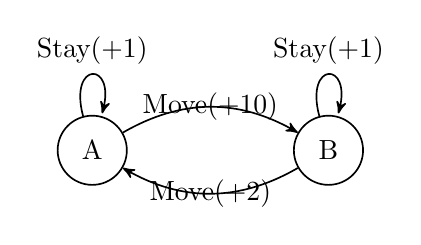
\begin{tikzpicture}[->, >=stealth', semithick, node distance=3cm]
    \node[state] (A) {A};
    \node[state] (B) [right of=A] {B};

    \path (A) edge [loop above] node {Stay(+1)} (A)
          (A) edge [bend left] node {Move(+10)} (B)
          (B) edge [loop above] node {Stay(+1)} (B)
          (B) edge [bend left] node {Move(+2)} (A);
\end{tikzpicture}
\end{center}

\textbf{1. Given:}
\begin{itemize}
    \item $\gamma=0.5$.
    \item $V_0(A)=0, V_0(B)=0$.
    \item Actions: Stay (R=1), Move (R=10 or 2).
\end{itemize}

\textbf{2. Formula:}
Value Iteration Update:
$$ V_{k+1}(s) = \max_{a} \left( R(s,a) + \gamma V_k(s') \right) $$

\textbf{3. Explanation:}
Unlike Policy Evaluation, Value Iteration assumes we greedily choose the best action at every step. We calculate the Q-value for every action and take the max.

\textbf{4. Calculation (State A):}
\textit{Option 1: Stay}
Reward = 1, Next State = A.
$$ Q(A, \text{Stay}) = 1 + 0.5 V_0(A) = 1 + 0 = 1 $$

\textit{Option 2: Move}
Reward = 10, Next State = B.
$$ Q(A, \text{Move}) = 10 + 0.5 V_0(B) = 10 + 0 = 10 $$

\textit{Maximize:}
$$ V_1(A) = \max(1, 10) = 10 $$

\textbf{Final Answer:}
$V_1(A) = 10$
\end{solutionbox}
\newpage

% Problem 1.10
\begin{problembox}{1.10: Grid World Probabilities}
A warehouse robot is in a grid cell (2,2). It attempts to move North.
- Success (moves N to (1,2)): 80\%
- Slip Left (moves W to (2,1)): 10\%
- Slip Right (moves E to (2,3)): 10\%
The rewards are: +5 for reaching (1,2), -1 for hitting a wall (assume (2,1) is a wall, robot bounces back to (2,2)), 0 otherwise.
Assume $\gamma=1$.
Calculate the expected immediate reward $R(s, \text{North})$.
\end{problembox}

\begin{guidebox}
Expected Reward = $\sum_{s'} p(s'|s,a) r(s,a,s')$.
\end{guidebox}

\begin{solutionbox}
\textbf{1. Given:}
\begin{itemize}
    \item Action: North.
    \item Outcome 1 (Success): Prob=0.8, Reward=+5.
    \item Outcome 2 (Slip/Wall): Prob=0.1, Reward=-1 (bounces).
    \item Outcome 3 (Slip/Empty): Prob=0.1, Reward=0.
\end{itemize}

\textbf{2. Formula:}
Expected Immediate Reward:
$$ E[R] = \sum_{outcome} P(outcome) \times R(outcome) $$

\textbf{3. Explanation:}
The transition function defines stochastic rewards. We must weight each possible reward by its probability of occurring.

\textbf{4. Calculation:}
$$ E[R] = (0.8 \times 5) + (0.1 \times -1) + (0.1 \times 0) $$
$$ E[R] = 4.0 - 0.1 + 0 $$
$$ E[R] = 3.9 $$

\textbf{Final Answer:}
$E[R] = 3.9$
\end{solutionbox}
\newpage

% Problem 1.11
\begin{problembox}{1.11: Infinite Horizon Return}
An agent receives a constant reward $R=2$ at every time step forever.
(a) If $\gamma=1$, what is the return $G_0$?
(b) If $\gamma=0.9$, what is the return $G_0$?
\end{problembox}

\begin{guidebox}
For infinite geometric series $\sum_{k=0}^\infty ar^k = \frac{a}{1-r}$ for $|r|<1$.
\end{guidebox}

\begin{solutionbox}
\textbf{1. Given:}
\begin{itemize}
    \item Constant Reward $R=2$.
    \item Time horizon: Infinite ($T=\infty$).
\end{itemize}

\textbf{2. Formula:}
$$ G_0 = \sum_{k=0}^{\infty} \gamma^k R = R + \gamma R + \gamma^2 R + \dots $$
This is a geometric series.
Sum $S = \frac{a}{1-r}$ where $a=R$ and $r=\gamma$.

\textbf{3. Calculation:}
\textit{Part (a): $\gamma=1$}
The series is $2 + 2 + 2 + \dots$.
Since $|r|=1$, the series diverges.
$$ G_0 = \infty $$

\textit{Part (b): $\gamma=0.9$}
Since $|\gamma| < 1$, the series converges.
$$ G_0 = \frac{R}{1-\gamma} $$
$$ G_0 = \frac{2}{1 - 0.9} = \frac{2}{0.1} $$
$$ G_0 = 20 $$

\textbf{Final Answer:}
(a) $\infty$
(b) $20$
\end{solutionbox}
\newpage

% Problem 1.12
\begin{problembox}{1.12: Comparing Policies}
State Space $S=\{s_1, s_2\}$.
Policy $\pi_1$: $V^{\pi_1}(s_1) = 10, V^{\pi_1}(s_2) = 5$.
Policy $\pi_2$: $V^{\pi_2}(s_1) = 8, V^{\pi_2}(s_2) = 6$.
Is $\pi_1 \ge \pi_2$ (strictly better or equal)? Why or why not?
\end{problembox}

\begin{guidebox}
A policy $\pi$ is defined to be better than or equal to $\pi'$ if $V_\pi(s) \ge V_{\pi'}(s)$ for \textbf{all} $s \in S$.
\end{guidebox}

\begin{solutionbox}
\textbf{1. Given:}
\begin{itemize}
    \item $V^{\pi_1} = [10, 5]$
    \item $V^{\pi_2} = [8, 6]$
\end{itemize}

\textbf{2. Definition:}
Partial Ordering of Policies: $\pi_1 \ge \pi_2 \iff V^{\pi_1}(s) \ge V^{\pi_2}(s)$ for all $s \in S$.

\textbf{3. Comparison:}
\textit{Check State $s_1$:}
$$ 10 \ge 8 \quad (\text{True, } \pi_1 \text{ is better}) $$

\textit{Check State $s_2$:}
$$ 5 \ge 6 \quad (\text{False, } \pi_1 \text{ is worse}) $$

\textbf{4. Conclusion:}
Since $\pi_1$ is not better than or equal to $\pi_2$ in *all* states (it is worse in $s_2$), we cannot say $\pi_1 \ge \pi_2$.

\textbf{Final Answer:}
No, $\pi_1$ is not strictly better. They are incomparable.
\end{solutionbox}
\newpage

% ----------------------------------------------------------------------
% TOPIC 2: TABULAR METHODS
% ----------------------------------------------------------------------
\section{Topic 2: Tabular Methods}
\textit{Topics Covered: Monte Carlo Methods, Temporal Difference Learning, SARSA, Q-Learning, n-Step TD, Eligibility Traces.}

% Problem 2.1
\begin{problembox}{2.1: Monte Carlo First-Visit vs Every-Visit}
Consider the following episode in an MDP with $\gamma=1$:
$S_1, R_1=1, S_2, R_2=2, S_1, R_3=3, S_3, R_4=0$ (Terminate).
Calculate the return $G_t$ for each visit to state $S_1$.
(a) What is the First-Visit return for $S_1$?
(b) What are the returns considered for Every-Visit MC for $S_1$?
\end{problembox}

\begin{guidebox}
The return $G_t$ is the sum of rewards from time $t$ onwards.
\end{guidebox}

\begin{solutionbox}
\textbf{1. Given:}
Trajectory: $S_1 \xrightarrow{1} S_2 \xrightarrow{2} S_1 \xrightarrow{3} S_3 \xrightarrow{0} \text{End}$.
Time steps of visits to $S_1$: $t=0$ and $t=2$.

\textbf{2. Formula:}
Return $G_t = \sum_{k=0}^{T-t-1} R_{t+k+1}$.

\textbf{3. Calculation:}
\textit{Calculate G for $t=0$ (First Visit):}
$$ G_0 = 1 + 2 + 3 + 0 = 6 $$

\textit{Calculate G for $t=2$ (Second Visit):}
$$ G_2 = 3 + 0 = 3 $$

\textbf{4. Final Answer:}
(a) First-Visit MC: Only considers the first occurrence. Return = \textbf{6}.
(b) Every-Visit MC: Considers all occurrences. Returns = \textbf{\{6, 3\}}.
\end{solutionbox}
\newpage

% Problem 2.2
\begin{problembox}{2.2: Incremental Monte Carlo Update}
You are estimating the value of state $A$.
Current estimate $V(A) = 10$. Number of visits $N(A) = 4$.
A new episode is observed with return $G = 20$ starting from $A$.
Calculate the new value $V(A)$ using the incremental mean update.
\end{problembox}

\begin{guidebox}
$V_{n+1} = V_n + \frac{1}{n+1}(G - V_n)$.
\end{guidebox}

\begin{solutionbox}
\textbf{1. Given:}
\begin{itemize}
    \item $V_{old} = 10$.
    \item $N_{old} = 4$.
    \item New Return $G = 20$.
\end{itemize}

\textbf{2. Formula:}
Incremental Mean:
$$ V_{new} = V_{old} + \frac{1}{N_{new}} (G - V_{old}) $$
Where $N_{new} = N_{old} + 1$.

\textbf{3. Explanation:}
Instead of storing all returns and re-averaging, we update the running mean by adding the error term $(G - V_{old})$ scaled by the step size $1/N$.

\textbf{4. Calculation:}
\textit{New Count:} $N_{new} = 4 + 1 = 5$.
$$ V_{new} = 10 + \frac{1}{5} (20 - 10) $$
$$ V_{new} = 10 + 0.2 (10) $$
$$ V_{new} = 10 + 2 = 12 $$

\textbf{Final Answer:}
$V(A) = 12$
\end{solutionbox}
\newpage

% Problem 2.3
\begin{problembox}{2.3: TD(0) Error Calculation}
An agent transitions from $S_t$ to $S_{t+1}$ receiving reward $R_{t+1} = -1$.
Current estimates: $V(S_t) = 5.0$, $V(S_{t+1}) = 4.5$.
Discount $\gamma = 0.9$.
Calculate the TD error $\delta_t$.
\end{problembox}

\begin{guidebox}
$\delta_t = R_{t+1} + \gamma V(S_{t+1}) - V(S_t)$.
\end{guidebox}

\begin{solutionbox}
\textbf{1. Given:}
\begin{itemize}
    \item $R_{t+1} = -1$.
    \item $V(S_t) = 5.0$.
    \item $V(S_{t+1}) = 4.5$.
    \item $\gamma = 0.9$.
\end{itemize}

\textbf{2. Formula:}
TD Error:
$$ \delta_t = \underbrace{R_{t+1} + \gamma V(S_{t+1})}_{\text{Target}} - \underbrace{V(S_t)}_{\text{Prediction}} $$

\textbf{3. Explanation:}
The TD error measures the difference between our new estimate (based on one step of real experience) and our old estimate.

\textbf{4. Calculation:}
\textit{Calculate Target:}
$$ Target = -1 + 0.9(4.5) = -1 + 4.05 = 3.05 $$

\textit{Calculate Error:}
$$ \delta_t = 3.05 - 5.0 = -1.95 $$

\textbf{Final Answer:}
$\delta_t = -1.95$
\end{solutionbox}
\newpage

% Problem 2.4
\begin{problembox}{2.4: TD(0) Value Update}
Using the TD error from Problem 2.3 ($\delta_t = -1.95$) and learning rate $\alpha = 0.1$, update the value of $V(S_t)$.
\end{problembox}

\begin{guidebox}
$V(S_t) \leftarrow V(S_t) + \alpha \delta_t$.
\end{guidebox}

\begin{solutionbox}
\textbf{1. Given:}
\begin{itemize}
    \item Old Value $V(S_t) = 5.0$.
    \item TD Error $\delta_t = -1.95$.
    \item Learning Rate $\alpha = 0.1$.
\end{itemize}

\textbf{2. Formula:}
TD Update Rule:
$$ V(S_t) \leftarrow V(S_t) + \alpha \delta_t $$

\textbf{3. Explanation:}
We shift the value function slightly towards the target. The learning rate controls the size of the step.

\textbf{4. Calculation:}
$$ V_{new} = 5.0 + 0.1(-1.95) $$
$$ V_{new} = 5.0 - 0.195 $$
$$ V_{new} = 4.805 $$

\textbf{Final Answer:}
$V(S_t) = 4.805$
\end{solutionbox}
\newpage

% Problem 2.5
\begin{problembox}{2.5: SARSA Update}
State $S$, Action $A$. Reward $R=2$, Next State $S'$, Next Action $A'$.
$Q(S,A) = 3.0, Q(S',A') = 4.5$.
$\alpha=0.1, \gamma=0.9$.
Calculate the new $Q(S,A)$ using the SARSA update rule.
\end{problembox}

\begin{guidebox}
$Q(S,A) \leftarrow Q(S,A) + \alpha [R + \gamma Q(S',A') - Q(S,A)]$.
\end{guidebox}

\begin{solutionbox}
\begin{center}
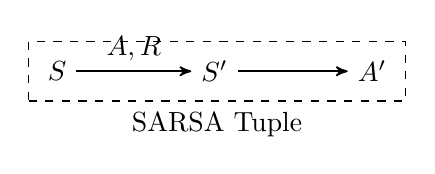
\begin{tikzpicture}[->, >=stealth', semithick, node distance=2cm]
    \node (s1) {$S$};
    \node (s2) [right of=s1] {$S'$};

    \path (s1) edge node [above] {$A, R$} (s2);
    \node [right of=s2] (a2) {$A'$};
    \path (s2) edge (a2);

    \node [draw, dashed, fit=(s1) (a2), label=below:SARSA Tuple] {};
\end{tikzpicture}
\end{center}

\textbf{1. Given:}
\begin{itemize}
    \item $R=2, \gamma=0.9, \alpha=0.1$.
    \item $Q(S,A)=3.0$.
    \item Next Q-value (actual action taken): $Q(S',A')=4.5$.
\end{itemize}

\textbf{2. Formula:}
SARSA (On-Policy) Update:
$$ Q(S,A) \leftarrow Q(S,A) + \alpha [ R + \gamma Q(S',A') - Q(S,A) ] $$

\textbf{3. Explanation:}
SARSA uses the quintuple $(S, A, R, S', A')$ to update the Q-value. It is "on-policy" because it uses the value of the action actually chosen by the policy ($A'$).

\textbf{4. Calculation:}
\textit{Calculate Target:}
$$ Target = 2 + 0.9(4.5) = 2 + 4.05 = 6.05 $$

\textit{Calculate TD Error:}
$$ \delta = 6.05 - 3.0 = 3.05 $$

\textit{Update Q:}
$$ Q_{new} = 3.0 + 0.1(3.05) $$
$$ Q_{new} = 3.0 + 0.305 = 3.305 $$

\textbf{Final Answer:}
$Q(S,A) = 3.305$
\end{solutionbox}
\newpage

% Problem 2.6
\begin{problembox}{2.6: Q-Learning Update}
Same setup as Problem 2.5, but using Q-Learning.
State $S$, Action $A$. Reward $R=2$, Next State $S'$.
Next state available actions: $\{A'_1, A'_2\}$.
$Q(S', A'_1) = 4.5, Q(S', A'_2) = 5.2$.
$Q(S,A) = 3.0, \alpha=0.1, \gamma=0.9$.
Calculate the new $Q(S,A)$.
\end{problembox}

\begin{guidebox}
$Q(S,A) \leftarrow Q(S,A) + \alpha [R + \gamma \max_{a'} Q(S',a') - Q(S,A)]$.
\end{guidebox}

\begin{solutionbox}
\textbf{1. Given:}
\begin{itemize}
    \item $R=2, \gamma=0.9, \alpha=0.1$.
    \item Current $Q(S,A)=3.0$.
    \item Next Q-values: $4.5$ and $5.2$.
\end{itemize}

\textbf{2. Formula:}
Q-Learning (Off-Policy) Update:
$$ Q(S,A) \leftarrow Q(S,A) + \alpha [ R + \gamma \max_{a'} Q(S',a') - Q(S,A) ] $$

\textbf{3. Explanation:}
Q-Learning updates towards the value of the *best possible* next action, regardless of what action the agent actually takes. This makes it an off-policy algorithm.

\textbf{4. Calculation:}
\textit{Find Max Next Q:}
$$ \max(4.5, 5.2) = 5.2 $$

\textit{Calculate Target:}
$$ Target = 2 + 0.9(5.2) = 2 + 4.68 = 6.68 $$

\textit{Update Q:}
$$ Q_{new} = 3.0 + 0.1(6.68 - 3.0) $$
$$ Q_{new} = 3.0 + 0.1(3.68) $$
$$ Q_{new} = 3.0 + 0.368 = 3.368 $$

\textbf{Final Answer:}
$Q(S,A) = 3.368$
\end{solutionbox}
\newpage

% Problem 2.7
\begin{problembox}{2.7: Expected SARSA}
State $S$, Action $A$. Reward $R=2$, Next State $S'$.
Policy $\pi$ at $S'$: 60\% chance to choose $A'_1$, 40\% chance to choose $A'_2$.
$Q(S', A'_1) = 4.5, Q(S', A'_2) = 5.2$.
$Q(S,A) = 3.0, \alpha=0.1, \gamma=0.9$.
Calculate the update target for Expected SARSA.
\end{problembox}

\begin{guidebox}
Target $= R + \gamma \sum_{a'} \pi(a'|S') Q(S',a')$.
\end{guidebox}

\begin{solutionbox}
\textbf{1. Given:}
\begin{itemize}
    \item Policy: $\pi(A'_1)=0.6, \pi(A'_2)=0.4$.
    \item Q-values: $Q(A'_1)=4.5, Q(A'_2)=5.2$.
    \item $R=2, \gamma=0.9$.
\end{itemize}

\textbf{2. Formula:}
Expected SARSA Target:
$$ Target = R + \gamma \sum_{a'} \pi(a'|S') Q(S',a') $$

\textbf{3. Explanation:}
Instead of using the max (Q-Learning) or a single sample (SARSA), Expected SARSA uses the *expected value* of the next state under the current policy. This reduces variance.

\textbf{4. Calculation:}
\textit{Calculate Expected Value of Next State $V(S')$:}
$$ V(S') = (0.6 \times 4.5) + (0.4 \times 5.2) $$
$$ V(S') = 2.7 + 2.08 = 4.78 $$

\textit{Calculate Target:}
$$ Target = 2 + 0.9(4.78) $$
$$ Target = 2 + 4.302 = 6.302 $$

\textbf{Final Answer:}
Target $= 6.302$
\end{solutionbox}
\newpage

% Problem 2.8
\begin{problembox}{2.8: Drone Cliff Walking}
A drone flies along a narrow canyon (Cliff Walking).
- Action 'Safe': moves to safe path, reward -1.
- Action 'Fall': crashes (falls off cliff), reward -100, returns to start.
Current Q-values: $Q(\text{Edge}, \text{Safe}) = -10, Q(\text{Edge}, \text{Fall}) = -50$.
$\epsilon=0.1$.
Calculate the expected return for one step from the 'Edge' state under an $\epsilon$-greedy policy.
\end{problembox}

\begin{guidebox}
$E[R] = \sum_a \pi(a|s) Q(s,a)$ is not quite right; we want expected *action value* (V) under the policy.
\end{guidebox}

\begin{solutionbox}
\begin{center}
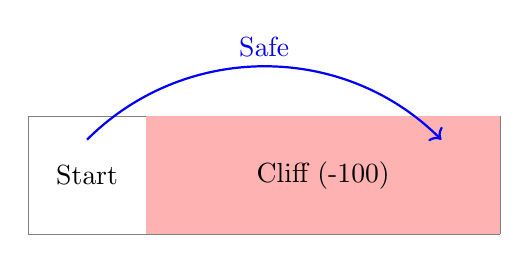
\begin{tikzpicture}[scale=1.5]
  \draw[step=1cm,gray,very thin] (0,0) grid (4,1);
  \fill[red!30] (1,0) rectangle (4,1);
  \node at (0.5,0.5) {Start};
  \node at (2.5,0.5) {Cliff (-100)};
  \draw[->, thick, blue] (0.5,0.8) to[out=45,in=135] node[above] {Safe} (3.5,0.8);
\end{tikzpicture}
\end{center}

\textbf{1. Given:}
\begin{itemize}
    \item Q-values: $Q(\text{Safe})=-10, Q(\text{Fall})=-50$.
    \item $\epsilon=0.1$.
    \item Number of actions $|A|=2$.
\end{itemize}

\textbf{2. Formula:}
Value of a state under policy $\pi$:
$$ V_\pi(s) = \sum_{a} \pi(a|s) Q(s,a) $$

\textbf{3. Explanation:}
We need to find the weighted average of the Q-values, where weights are the probabilities of taking each action under the $\epsilon$-greedy policy.

\textbf{4. Calculation:}
\textit{Determine Probabilities:}
Greedy action is 'Safe' (since $-10 > -50$).
$$ \pi(\text{Safe}) = 1 - \epsilon + \frac{\epsilon}{2} = 0.9 + 0.05 = 0.95 $$
$$ \pi(\text{Fall}) = \frac{\epsilon}{2} = 0.05 $$

\textit{Calculate Expectation:}
$$ V = (0.95 \times -10) + (0.05 \times -50) $$
$$ V = -9.5 + (-2.5) $$
$$ V = -12.0 $$

\textbf{Final Answer:}
$V_\pi(\text{Edge}) = -12.0$
\end{solutionbox}
\newpage

% Problem 2.9
\begin{problembox}{2.9: n-Step TD Return}
Calculate the 2-step return $G_{t:t+2}$ for the sequence:
$S_t, R_{t+1}=1, S_{t+1}, R_{t+2}=2, S_{t+2}$.
Given $V(S_{t+2}) = 10, \gamma=0.9$.
\end{problembox}

\begin{guidebox}
$G_{t:t+n} = R_{t+1} + \gamma R_{t+2} + \dots + \gamma^{n-1} R_{t+n} + \gamma^n V(S_{t+n})$.
\end{guidebox}

\begin{solutionbox}
\textbf{1. Given:}
\begin{itemize}
    \item Rewards: $R_{t+1}=1, R_{t+2}=2$.
    \item Estimated Value: $V(S_{t+2})=10$.
    \item Discount $\gamma=0.9$.
    \item Steps $n=2$.
\end{itemize}

\textbf{2. Formula:}
n-Step Return:
$$ G_{t:t+n} = R_{t+1} + \gamma R_{t+2} + \dots + \gamma^{n-1} R_{t+n} + \gamma^n V(S_{t+n}) $$

\textbf{3. Explanation:}
This method looks ahead $n$ steps using real rewards, then bootstraps using the estimated value of the state reached after $n$ steps. It bridges the gap between MC (full return) and TD(0) (1-step return).

\textbf{4. Calculation:}
$$ G = 1 + \gamma(2) + \gamma^2(10) $$
$$ G = 1 + 0.9(2) + (0.9)^2(10) $$
$$ G = 1 + 1.8 + 0.81(10) $$
$$ G = 2.8 + 8.1 = 10.9 $$

\textbf{Final Answer:}
$G_{t:t+2} = 10.9$
\end{solutionbox}
\newpage

% Problem 2.10
\begin{problembox}{2.10: Double Q-Learning}
We have two Q-tables $Q_1$ and $Q_2$.
Current state $S$, Action $A$, Reward $R$, Next state $S'$.
Update $Q_1(S,A)$.
$Q_1(S,A)=3, Q_2(S,A)=3$.
In state $S'$, $Q_1$ suggests best action is $A'_1$ (value 10), but $Q_2(S', A'_1) = 8$.
$R=1, \gamma=0.9, \alpha=0.1$.
\end{problembox}

\begin{guidebox}
Update $Q_1$ using the value of the action maximizing $Q_1$, but taken from $Q_2$.
Target $= R + \gamma Q_2(S', \arg\max_a Q_1(S', a))$.
\end{guidebox}

\begin{solutionbox}
\textbf{1. Given:}
\begin{itemize}
    \item Update target: $Q_1(S,A)$.
    \item Max action in $S'$ according to $Q_1$: $A^* = A'_1$.
    \item Value of $A^*$ in $Q_2$: $Q_2(S', A'_1) = 8$.
    \item $R=1, \gamma=0.9, \alpha=0.1$.
    \item Current $Q_1(S,A) = 3$.
\end{itemize}

\textbf{2. Formula:}
Double Q-Learning Target for $Q_1$:
$$ Y = R + \gamma Q_2(S', \arg\max_a Q_1(S', a)) $$

\textbf{3. Explanation:}
Standard Q-Learning overestimates values because it takes the max over noisy estimates. Double Q-Learning decouples selection (using $Q_1$) from evaluation (using $Q_2$) to reduce bias.

\textbf{4. Calculation:}
\textit{Calculate Target:}
$$ Y = 1 + 0.9(8) = 1 + 7.2 = 8.2 $$

\textit{Update $Q_1$:}
$$ Q_1(S,A) \leftarrow 3 + 0.1(8.2 - 3) $$
$$ Q_1(S,A) \leftarrow 3 + 0.1(5.2) $$
$$ Q_1(S,A) \leftarrow 3 + 0.52 = 3.52 $$

\textbf{Final Answer:}
$Q_1(S,A) = 3.52$
\end{solutionbox}
\newpage

% Problem 2.11
\begin{problembox}{2.11: Eligibility Trace Accumulation}
An accumulating trace $e_t(s)$ is used with $\lambda=0.5, \gamma=0.9$.
At $t=0$, $e_0(s)=0$.
At $t=1$, state $s$ is visited.
At $t=2$, state $s$ is visited again.
Calculate $e_2(s)$ just after the visit.
\end{problembox}

\begin{guidebox}
$e_t(s) = \gamma \lambda e_{t-1}(s) + \mathbf{1}(S_t=s)$.
\end{guidebox}

\begin{solutionbox}
\textbf{1. Given:}
\begin{itemize}
    \item Decay rate $\gamma \lambda = 0.9 \times 0.5 = 0.45$.
    \item Visits at $t=1$ and $t=2$.
\end{itemize}

\textbf{2. Formula:}
Accumulating Trace Update:
$$ e_t(s) = \gamma \lambda e_{t-1}(s) + 1 $$
(if $S_t=s$).

\textbf{3. Explanation:}
Eligibility traces keep a memory of visited states. "Accumulating" means we add +1 every time we visit, allowing the trace to grow > 1.

\textbf{4. Calculation:}
\textit{At $t=1$ (First Visit):}
$$ e_1(s) = 0.45(0) + 1 = 1.0 $$

\textit{At $t=2$ (Second Visit):}
Decay the previous value, then add 1.
$$ e_2(s) = 0.45(1.0) + 1 $$
$$ e_2(s) = 0.45 + 1 = 1.45 $$

\textbf{Final Answer:}
$e_2(s) = 1.45$
\end{solutionbox}
\newpage

% Problem 2.12
\begin{problembox}{2.12: TD($\lambda$) Update}
Using the trace $e_2(s)=1.45$ from Problem 2.11.
Suppose at $t=2$ a TD error $\delta_2 = 2.0$ occurs.
Update $V(s)$ given $\alpha=0.1$.
\end{problembox}

\begin{guidebox}
$\Delta V(s) = \alpha \delta_t e_t(s)$.
\end{guidebox}

\begin{solutionbox}
\textbf{1. Given:}
\begin{itemize}
    \item TD Error $\delta = 2.0$.
    \item Trace $e(s) = 1.45$.
    \item Learning Rate $\alpha = 0.1$.
\end{itemize}

\textbf{2. Formula:}
$$ V(s) \leftarrow V(s) + \alpha \delta e(s) $$

\textbf{3. Explanation:}
In TD($\lambda$), we update all states in the trace, not just the current one. The update is proportional to how "eligible" (recently/frequently visited) the state is.

\textbf{4. Calculation:}
$$ \Delta V = 0.1 \times 2.0 \times 1.45 $$
$$ \Delta V = 0.2 \times 1.45 $$
$$ \Delta V = 0.29 $$

\textbf{Final Answer:}
Increase $V(s)$ by $0.29$.
\end{solutionbox}
\newpage

% ----------------------------------------------------------------------
% TOPIC 3: VALUE FUNCTION APPROXIMATION & DEEP RL
% ----------------------------------------------------------------------
\section{Topic 3: Value Function Approximation \& Deep RL}
\textit{Topics Covered: Linear Function Approximation, Gradient Descent, Deep Q-Networks (DQN), Loss Functions, Experience Replay, Policy Gradients.}

% Problem 3.1
\begin{problembox}{3.1: Linear Value Prediction}
State $s$ is represented by a feature vector $\mathbf{x}(s) = [0.5, 1.0, -0.2]^T$.
The current weight vector is $\mathbf{w} = [2.0, -1.0, 3.0]^T$.
Calculate the estimated value $\hat{v}(s, \mathbf{w}) = \mathbf{w}^T \mathbf{x}(s)$.
\end{problembox}

\begin{guidebox}
Perform the dot product: $w_1 x_1 + w_2 x_2 + w_3 x_3$.
\end{guidebox}

\begin{solutionbox}
\textbf{1. Given:}
\begin{itemize}
    \item Features $\mathbf{x} = [0.5, 1.0, -0.2]$.
    \item Weights $\mathbf{w} = [2.0, -1.0, 3.0]$.
\end{itemize}

\textbf{2. Formula:}
Linear Approximation:
$$ \hat{v}(s) = \sum w_i x_i $$

\textbf{3. Explanation:}
The value is estimated as a weighted sum of the features.

\textbf{4. Calculation:}
$$ \hat{v} = (2.0)(0.5) + (-1.0)(1.0) + (3.0)(-0.2) $$
$$ \hat{v} = 1.0 - 1.0 - 0.6 $$
$$ \hat{v} = -0.6 $$

\textbf{Final Answer:}
$\hat{v}(s) = -0.6$
\end{solutionbox}
\newpage

% Problem 3.2
\begin{problembox}{3.2: Linear SGD Update}
Using the result from Problem 3.1 ($\hat{v}(s) = -0.6$).
Suppose the true target value is $v_\pi(s) = 1.0$.
Perform one SGD update on $\mathbf{w}$ with step size $\alpha = 0.1$.
\end{problembox}

\begin{guidebox}
$\mathbf{w} \leftarrow \mathbf{w} + \alpha [v_\pi(s) - \hat{v}(s)] \mathbf{x}(s)$.
\end{guidebox}

\begin{solutionbox}
\textbf{1. Given:}
\begin{itemize}
    \item Prediction $\hat{v} = -0.6$.
    \item Target $v_\pi = 1.0$.
    \item Error $\delta = 1.0 - (-0.6) = 1.6$.
    \item $\mathbf{x} = [0.5, 1.0, -0.2]^T$.
\end{itemize}

\textbf{2. Formula:}
Gradient Descent Update:
$$ \mathbf{w} \leftarrow \mathbf{w} + \alpha (Target - Prediction) \mathbf{x} $$

\textbf{3. Explanation:}
We move the weights in the direction of the features $\mathbf{x}$ to reduce the error.

\textbf{4. Calculation:}
Scale of update: $\alpha \delta = 0.1 \times 1.6 = 0.16$.
Update vector:
$$ 0.16 \times [0.5, 1.0, -0.2] = [0.08, 0.16, -0.032] $$

Add to original weights:
$$ w_1 = 2.0 + 0.08 = 2.08 $$
$$ w_2 = -1.0 + 0.16 = -0.84 $$
$$ w_3 = 3.0 - 0.032 = 2.968 $$

\textbf{Final Answer:}
$\mathbf{w}_{new} = [2.08, -0.84, 2.968]^T$
\end{solutionbox}
\newpage

% Problem 3.3
\begin{problembox}{3.3: Pong AI Q-Network}
An AI playing Pong uses a simple Q-network.
- Input state $x = [1, 0]$ (simplified feature).
- Hidden Layer $h$ (ReLU): Weights $W_1 = [[0.5, -0.2], [0.1, 0.8]]$ (2x2 matrix).
- Output Layer $Q$ (Linear): Weights $W_2 = [1.0, -1.0]$ (1x2 matrix, one output for action $a$).
Calculate $Q(s,a)$. Note: ReLU(z) = max(0, z).
\end{problembox}

\begin{guidebox}
1. $z = W_1 x$. 2. $h = \text{ReLU}(z)$. 3. $Q = W_2 h$.
\end{guidebox}

\begin{solutionbox}
\begin{center}
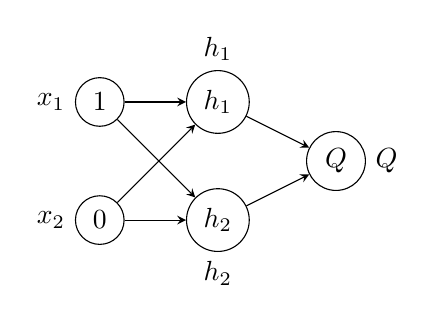
\begin{tikzpicture}[x=1.5cm, y=1.5cm, >=stealth]
  \node[circle,draw,label=left:$x_1$] (I1) at (0,1) {1};
  \node[circle,draw,label=left:$x_2$] (I2) at (0,0) {0};

  \node[circle,draw,label=above:$h_1$] (H1) at (1,1) {$h_1$};
  \node[circle,draw,label=below:$h_2$] (H2) at (1,0) {$h_2$};

  \node[circle,draw,label=right:$Q$] (O) at (2,0.5) {$Q$};

  \draw[->] (I1) -- (H1); \draw[->] (I1) -- (H2);
  \draw[->] (I2) -- (H1); \draw[->] (I2) -- (H2);
  \draw[->] (H1) -- (O); \draw[->] (H2) -- (O);
\end{tikzpicture}
\end{center}

\textbf{1. Given:}
\begin{itemize}
    \item Input $x=[1, 0]^T$.
    \item $W_1 = [[0.5, -0.2], [0.1, 0.8]]$.
    \item $W_2 = [1.0, -1.0]$.
\end{itemize}

\textbf{2. Formula:}
Forward Pass:
$$ h = \text{ReLU}(W_1 x) $$
$$ Q = W_2 h $$

\textbf{3. Explanation:}
A standard feed-forward pass. We multiply inputs by weights, apply non-linearity, then combine for the output.

\textbf{4. Calculation:}
\textit{Hidden Layer Pre-activation:}
$$ z_1 = 0.5(1) + (-0.2)(0) = 0.5 $$
$$ z_2 = 0.1(1) + 0.8(0) = 0.1 $$

\textit{ReLU Activation:}
$$ h_1 = \max(0, 0.5) = 0.5 $$
$$ h_2 = \max(0, 0.1) = 0.1 $$

\textit{Output Layer:}
$$ Q = 1.0(h_1) - 1.0(h_2) $$
$$ Q = 1.0(0.5) - 1.0(0.1) = 0.4 $$

\textbf{Final Answer:}
$Q(s,a) = 0.4$
\end{solutionbox}
\newpage

% Problem 3.4
\begin{problembox}{3.4: DQN Loss Calculation}
Current Q-network prediction $Q(s,a; \theta) = 3.5$.
Target Network prediction $Q(s', a'; \theta^-) = 4.0$.
Reward $R=1, \gamma=0.9$.
Calculate the Squared Bellman Error Loss $L = \frac{1}{2}(y - Q)^2$.
\end{problembox}

\begin{guidebox}
Target $y = R + \gamma \max_{a'} Q(s', a'; \theta^-)$. Assume the given value is already the max.
\end{guidebox}

\begin{solutionbox}
\textbf{1. Given:}
\begin{itemize}
    \item Prediction $Q_{pred} = 3.5$.
    \item Max Next Q $Q_{next} = 4.0$.
    \item $R=1, \gamma=0.9$.
\end{itemize}

\textbf{2. Formula:}
DQN Target:
$$ y = R + \gamma \max_{a'} Q(s', a'; \theta^-) $$
Loss:
$$ L = \frac{1}{2} (y - Q_{pred})^2 $$

\textbf{3. Explanation:}
DQN treats the Right Hand Side of the Bellman equation (computed with a frozen target network) as the ground truth label $y$ for a regression problem.

\textbf{4. Calculation:}
\textit{Calculate Target y:}
$$ y = 1 + 0.9(4.0) = 1 + 3.6 = 4.6 $$

\textit{Calculate Error:}
$$ \delta = 4.6 - 3.5 = 1.1 $$

\textit{Calculate Loss:}
$$ L = 0.5 (1.1)^2 = 0.5 (1.21) = 0.605 $$

\textbf{Final Answer:}
$L = 0.605$
\end{solutionbox}
\newpage

% Problem 3.5
\begin{problembox}{3.5: Gradient Descent Step}
Given the loss gradient $\nabla_\theta L = 2.4$ and current parameter $\theta = 0.5$.
Perform one gradient descent update with learning rate $\alpha=0.01$.
\end{problembox}

\begin{guidebox}
$\theta \leftarrow \theta - \alpha \nabla_\theta L$.
\end{guidebox}

\begin{solutionbox}
\textbf{1. Given:}
\begin{itemize}
    \item Gradient $g = 2.4$.
    \item Parameter $\theta = 0.5$.
    \item Learning rate $\alpha = 0.01$.
\end{itemize}

\textbf{2. Formula:}
$$ \theta_{new} = \theta_{old} - \alpha \nabla_\theta L $$

\textbf{3. Explanation:}
We subtract the gradient to move down the slope of the loss landscape, minimizing the loss.

\textbf{4. Calculation:}
$$ \theta_{new} = 0.5 - 0.01(2.4) $$
$$ \theta_{new} = 0.5 - 0.024 $$
$$ \theta_{new} = 0.476 $$

\textbf{Final Answer:}
$\theta_{new} = 0.476$
\end{solutionbox}
\newpage

% Problem 3.6
\begin{problembox}{3.6: Experience Replay Buffer}
A replay buffer has capacity $N=1000$.
We store transitions $(S_t, A_t, R_{t+1}, S_{t+1})$ every step.
If we train for 5000 steps, how many times has the buffer been overwritten (completely filled and wrapped around)?
\end{problembox}

\begin{guidebox}
Number of wraps = Total Steps / Capacity.
\end{guidebox}

\begin{solutionbox}
\textbf{1. Given:}
\begin{itemize}
    \item Capacity $C=1000$.
    \item Steps $T=5000$.
\end{itemize}

\textbf{2. Formula:}
$$ \text{Wraps} = \lfloor \frac{T}{C} \rfloor $$

\textbf{3. Explanation:}
The buffer works as a First-In-First-Out (FIFO) queue (or circular buffer). Once it hits 1000, new data overwrites the oldest data.

\textbf{4. Calculation:}
$$ \frac{5000}{1000} = 5 $$
It filled up once (step 1000), then overwrote itself 4 more times (steps 2000, 3000, 4000, 5000).
Total cycles completed = 5.

\textbf{Final Answer:}
5 times.
\end{solutionbox}
\newpage

% Problem 3.7
\begin{problembox}{3.7: Huber Loss}
Calculate the Huber Loss for an error $\delta = 1.5$ with threshold $\delta_{check} = 1.0$.
Formula: $L_\delta = \begin{cases} 0.5 \delta^2 & |\delta| \le 1 \\ |\delta| - 0.5 & |\delta| > 1 \end{cases}$.
\end{problembox}

\begin{guidebox}
Check if $|\delta| > 1$.
\end{guidebox}

\begin{solutionbox}
\textbf{1. Given:}
\begin{itemize}
    \item Error $\delta = 1.5$.
    \item Threshold = 1.0.
\end{itemize}

\textbf{2. Formula:}
Since $|\delta| = 1.5 > 1$, we use the linear component:
$$ L = |\delta| - 0.5 $$

\textbf{3. Explanation:}
Huber loss is robust to outliers. For small errors, it acts like MSE (quadratic). For large errors, it acts like MAE (linear) to prevent exploding gradients.

\textbf{4. Calculation:}
$$ L = 1.5 - 0.5 = 1.0 $$

\textbf{Final Answer:}
$L = 1.0$
\end{solutionbox}
\newpage

% Problem 3.8
\begin{problembox}{3.8: Double DQN Target}
State $S'$, Actions $\{a_1, a_2\}$.
Online Net $Q_\theta$: $Q(S', a_1) = 3.0, Q(S', a_2) = 4.0$.
Target Net $Q_{\theta^-}$: $Q(S', a_1) = 2.5, Q(S', a_2) = 2.0$.
Reward $R=1, \gamma=0.9$.
Calculate the Double DQN Target $y$.
\end{problembox}

\begin{guidebox}
$y = R + \gamma Q_{\theta^-}(S', \arg\max_a Q_\theta(S', a))$.
\end{guidebox}

\begin{solutionbox}
\textbf{1. Given:}
\begin{itemize}
    \item Online Q: $[3.0, 4.0]$.
    \item Target Q: $[2.5, 2.0]$.
    \item $R=1, \gamma=0.9$.
\end{itemize}

\textbf{2. Formula:}
$$ y = R + \gamma Q_{target}(S', \arg\max_a Q_{online}(S', a)) $$

\textbf{3. Explanation:}
We pick the best action using the Online network (greedy selection) but evaluate its value using the Target network (unbiased evaluation).

\textbf{4. Calculation:}
\textit{Selection (Online):}
$\max(3.0, 4.0)$ is $4.0$, which corresponds to action $a_2$.

\textit{Evaluation (Target):}
Look up $a_2$ in Target Net: $Q_{target}(S', a_2) = 2.0$.

\textit{Compute Y:}
$$ y = 1 + 0.9(2.0) = 1 + 1.8 = 2.8 $$

\textbf{Final Answer:}
$y = 2.8$
\end{solutionbox}
\newpage

% Problem 3.9
\begin{problembox}{3.9: Dueling DQN Architecture}
A Dueling DQN outputs Value $V(s) = 5.0$ and Advantages $A(s, a_1) = -0.5, A(s, a_2) = 0.5$.
Using the simple aggregation $Q(s,a) = V(s) + A(s,a)$, calculate $Q(s, a_1)$ and $Q(s, a_2)$.
\end{problembox}

\begin{guidebox}
Just add them up.
\end{guidebox}

\begin{solutionbox}
\begin{center}
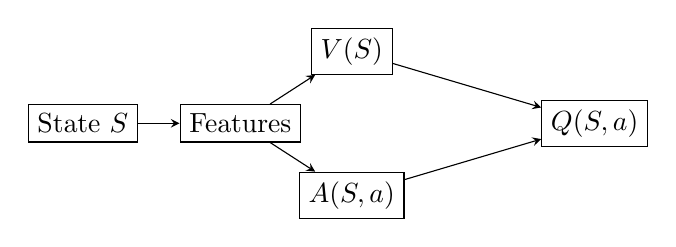
\begin{tikzpicture}[>=stealth, node distance=2cm]
    \node[draw] (input) {State $S$};
    \node[draw, right of=input] (shared) {Features};

    \node[draw, above right of=shared, yshift=-0.5cm] (val) {$V(S)$};
    \node[draw, below right of=shared, yshift=0.5cm] (adv) {$A(S,a)$};

    \node[draw, right of=shared, xshift=2.5cm] (q) {$Q(S,a)$};

    \draw[->] (input) -- (shared);
    \draw[->] (shared) -- (val);
    \draw[->] (shared) -- (adv);
    \draw[->] (val) -- (q);
    \draw[->] (adv) -- (q);
\end{tikzpicture}
\end{center}

\textbf{1. Given:}
\begin{itemize}
    \item $V(s) = 5.0$.
    \item $A(s, a_1) = -0.5$.
    \item $A(s, a_2) = 0.5$.
\end{itemize}

\textbf{2. Formula:}
$$ Q(s,a) = V(s) + A(s,a) $$

\textbf{3. Explanation:}
Dueling DQN splits the network into a stream estimating the state value (how good is it to be here?) and a stream estimating the advantage (how much better is this action than the average?).

\textbf{4. Calculation:}
$$ Q(s, a_1) = 5.0 + (-0.5) = 4.5 $$
$$ Q(s, a_2) = 5.0 + 0.5 = 5.5 $$

\textbf{Final Answer:}
$Q(a_1)=4.5, Q(a_2)=5.5$
\end{solutionbox}
\newpage

% Problem 3.10
\begin{problembox}{3.10: Prioritized Replay Probability}
Two transitions in buffer.
Transition 1: TD Error $\delta_1 = 2.0$.
Transition 2: TD Error $\delta_2 = 1.0$.
Exponent $\alpha = 1$ (proportional).
Calculate the probability $P(1)$ of sampling Transition 1.
\end{problembox}

\begin{guidebox}
$P(i) = |\delta_i|^\alpha / \sum |\delta_j|^\alpha$.
\end{guidebox}

\begin{solutionbox}
\textbf{1. Given:}
\begin{itemize}
    \item Errors: $|\delta_1|=2.0, |\delta_2|=1.0$.
    \item Exponent $\alpha=1$.
\end{itemize}

\textbf{2. Formula:}
$$ P(i) = \frac{p_i^\alpha}{\sum_k p_k^\alpha} $$
where priority $p_i = |\delta_i|$.

\textbf{3. Explanation:}
Prioritized Replay samples important transitions (high error) more frequently. $P(i)$ is the normalized probability.

\textbf{4. Calculation:}
Sum of priorities: $2.0 + 1.0 = 3.0$.
$$ P(1) = \frac{2.0}{3.0} \approx 0.667 $$
$$ P(2) = \frac{1.0}{3.0} \approx 0.333 $$

\textbf{Final Answer:}
$P(1) \approx 0.67$
\end{solutionbox}
\newpage

% Problem 3.11
\begin{problembox}{3.11: Policy Gradient (REINFORCE)}
Trajectory $\tau$: Action $a_t$ taken.
Return $G_t = 10$.
Policy Output $\pi(a_t|s_t) = 0.2$.
Calculate $\nabla_\theta J(\theta)$ approximation using $\nabla \ln \pi = \frac{1}{\pi} \nabla \pi$.
Assume $\nabla_\theta \pi(a_t|s_t) = 0.05$.
\end{problembox}

\begin{guidebox}
$\nabla J \approx G_t \nabla \ln \pi(a_t|s_t) = G_t \frac{\nabla \pi}{\pi}$.
\end{guidebox}

\begin{solutionbox}
\textbf{1. Given:}
\begin{itemize}
    \item Return $G_t = 10$.
    \item Probability $\pi = 0.2$.
    \item Gradient of prob $\nabla \pi = 0.05$.
\end{itemize}

\textbf{2. Formula:}
Policy Gradient Theorem (REINFORCE sample):
$$ \nabla J \approx G_t \nabla \ln \pi(a_t|s_t) $$
Using log derivative trick $\nabla \ln x = \frac{\nabla x}{x}$:
$$ \nabla J \approx G_t \frac{\nabla \pi}{\pi} $$

\textbf{3. Explanation:}
We increase the probability of action $a_t$ proportional to the return $G_t$. The term $\frac{1}{\pi}$ scales it inversely by probability (rare actions get bigger boosts).

\textbf{4. Calculation:}
\textit{Score Function:}
$$ \nabla \ln \pi = \frac{0.05}{0.2} = 0.25 $$

\textit{Total Gradient:}
$$ 10 \times 0.25 = 2.5 $$

\textbf{Final Answer:}
$\nabla J = 2.5$
\end{solutionbox}
\newpage

% Problem 3.12
\begin{problembox}{3.12: Actor-Critic Update}
Critic Error $\delta = 1.5$.
Actor chooses action $a$ with probability $0.5$.
Compatible feature $\psi(s,a) = \nabla \ln \pi(a|s) = [0.1, -0.1]^T$.
Update actor weights $\theta$ with $\alpha=0.1$.
\end{problembox}

\begin{guidebox}
$\theta \leftarrow \theta + \alpha \delta \psi(s,a)$.
\end{guidebox}

\begin{solutionbox}
\textbf{1. Given:}
\begin{itemize}
    \item TD Error $\delta = 1.5$.
    \item Score vector $\psi = [0.1, -0.1]^T$.
    \item Learning rate $\alpha = 0.1$.
\end{itemize}

\textbf{2. Formula:}
Actor Update:
$$ \theta_{new} = \theta + \alpha \delta \nabla \ln \pi $$

\textbf{3. Explanation:}
Similar to REINFORCE, but uses the Critic's TD error $\delta$ instead of the full return $G_t$ to reduce variance.

\textbf{4. Calculation:}
$$ \Delta \theta = 0.1 \times 1.5 \times [0.1, -0.1] $$
$$ \Delta \theta = 0.15 \times [0.1, -0.1] $$
$$ \Delta \theta = [0.015, -0.015] $$

\textbf{Final Answer:}
Update vector is $[0.015, -0.015]^T$.
\end{solutionbox}
\newpage

% ----------------------------------------------------------------------
% TOPIC 4: MODEL-BASED & ADVANCED
% ----------------------------------------------------------------------
\section{Topic 4: Model-Based \& Advanced}
\textit{Topics Covered: Monte Carlo Tree Search (MCTS), AlphaGo, AlphaZero, MuZero, Model-Based RL, Dyna-Q.}

% Problem 4.1
\begin{problembox}{4.1: MCTS UCT Calculation}
In an AlphaGo-like game tree search, a node $s$ has been visited $N(s) = 50$ times.
It has two children actions:
- Action $a_1$: $N(s, a_1) = 10, Q(s, a_1) = 0.6$.
- Action $a_2$: $N(s, a_2) = 40, Q(s, a_2) = 0.8$.
Exploration constant $c_{uct} = \sqrt{2}$.
Calculate the UCT value for $a_1$.
\end{problembox}

\begin{guidebox}
$UCT(s,a) = Q(s,a) + c \sqrt{\frac{\ln N(s)}{N(s,a)}}$.
\end{guidebox}

\begin{solutionbox}
\begin{center}
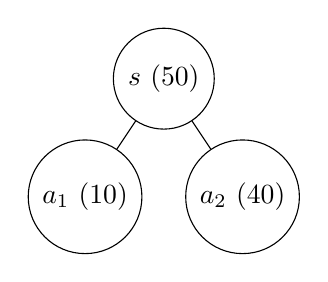
\begin{tikzpicture}[level/.style={sibling distance=20mm}]
\node [circle,draw] (z){$s$ (50)}
  child {node [circle,draw] (a) {$a_1$ (10)}}
  child {node [circle,draw] (b) {$a_2$ (40)}};
\end{tikzpicture}
\end{center}

\textbf{1. Given:}
\begin{itemize}
    \item Parent visits $N=50$.
    \item Child $a_1$: $n=10, Q=0.6$.
    \item $c = \sqrt{2} \approx 1.414$.
\end{itemize}

\textbf{2. Formula:}
$$ UCT = Q + c \sqrt{\frac{\ln N}{n}} $$

\textbf{3. Explanation:}
UCT treats tree search as a bandit problem at every node. We select children with high value ($Q$) or high uncertainty (low $n$).

\textbf{4. Calculation:}
\textit{Log term:} $\ln(50) \approx 3.912$.
\textit{Ratio:} $3.912 / 10 = 0.3912$.
\textit{Square Root:} $\sqrt{0.3912} \approx 0.625$.
\textit{Exploration Bonus:} $1.414 \times 0.625 \approx 0.884$.
\textit{Total:} $0.6 + 0.884 = 1.484$.

\textbf{Final Answer:}
$UCT(a_1) = 1.484$
\end{solutionbox}
\newpage

% Problem 4.2
\begin{problembox}{4.2: MCTS Selection}
Using the same setup as Problem 4.1.
Calculate the UCT value for $a_2$ and determine which action is selected.
\end{problembox}

\begin{guidebox}
Calculate $UCT(a_2)$ and compare with $UCT(a_1)$.
\end{guidebox}

\begin{solutionbox}
\textbf{1. Given:}
\begin{itemize}
    \item Parent $N=50$.
    \item Child $a_2$: $n=40, Q=0.8$.
    \item $c = 1.414$.
\end{itemize}

\textbf{2. Calculation:}
\textit{Log term:} $\ln(50) \approx 3.912$.
\textit{Ratio:} $3.912 / 40 \approx 0.0978$.
\textit{Square Root:} $\sqrt{0.0978} \approx 0.313$.
\textit{Exploration Bonus:} $1.414 \times 0.313 \approx 0.442$.
\textit{Total:} $0.8 + 0.442 = 1.242$.

\textbf{3. Comparison:}
$UCT(a_1) = 1.484$ (from prev problem).
$UCT(a_2) = 1.242$.
Since $1.484 > 1.242$, we select $a_1$.

\textbf{Final Answer:}
$a_1$ is selected.
\end{solutionbox}
\newpage

% Problem 4.3
\begin{problembox}{4.3: MCTS Backpropagation}
A simulation starting from node $s_{leaf}$ results in a return $G = 1$.
The path from root to leaf is $s_{root} \rightarrow a_1 \rightarrow s_1 \rightarrow a_2 \rightarrow s_{leaf}$.
Current statistics:
- $s_{root}: N=10, Q=0.5$.
- $s_1: N=5, Q=0.4$.
Update the values for $s_1$.
\end{problembox}

\begin{guidebox}
$N \leftarrow N + 1$.
$Q \leftarrow Q + \frac{1}{N}(G - Q)$.
\end{guidebox}

\begin{solutionbox}
\textbf{1. Given:}
\begin{itemize}
    \item Node $s_1$ old stats: $N=5, Q=0.4$.
    \item New result $G=1$.
\end{itemize}

\textbf{2. Formula:}
Update Count: $N_{new} = N_{old} + 1$.
Update Mean:
$$ Q_{new} = Q_{old} + \frac{1}{N_{new}}(G - Q_{old}) $$

\textbf{3. Explanation:}
Backpropagation updates the statistics of all nodes traversed during the selection phase.

\textbf{4. Calculation:}
\textit{New Count:} $N = 5 + 1 = 6$.
\textit{New Value:}
$$ Q = 0.4 + \frac{1}{6}(1 - 0.4) $$
$$ Q = 0.4 + \frac{0.6}{6} $$
$$ Q = 0.4 + 0.1 = 0.5 $$

\textbf{Final Answer:}
$N=6, Q=0.5$
\end{solutionbox}
\newpage

% Problem 4.4
\begin{problembox}{4.4: AlphaGo Value Network}
The value network $v_\theta(s)$ predicts the probability of winning from state $s$.
Output is a scalar in $[-1, 1]$ (using tanh) or $[0, 1]$ (using sigmoid). Let's assume tanh.
If the network outputs $0.8$, what does this imply about the win probability?
\end{problembox}

\begin{guidebox}
Map $[-1, 1]$ to probability. $P(\text{Win}) = \frac{v + 1}{2}$.
\end{guidebox}

\begin{solutionbox}
\textbf{1. Given:}
\begin{itemize}
    \item Network output $v = 0.8$ (range $[-1, 1]$).
    \item Mapping: -1 (Loss) to +1 (Win).
\end{itemize}

\textbf{2. Formula:}
$$ P(\text{Win}) = \frac{v - (-1)}{1 - (-1)} = \frac{v+1}{2} $$

\textbf{3. Explanation:}
We linearly scale the range $[-1, 1]$ to the probability range $[0, 1]$.

\textbf{4. Calculation:}
$$ P = \frac{0.8 + 1}{2} = \frac{1.8}{2} = 0.9 $$

\textbf{Final Answer:}
Win Probability = 90\%
\end{solutionbox}
\newpage

% Problem 4.5
\begin{problembox}{4.5: AlphaZero Loss Function}
Given a training example $(s, \pi_{MCTS}, z)$.
- MCTS Policy $\pi_{MCTS} = [0.2, 0.8]$.
- Neural Net Policy $p_\theta = [0.4, 0.6]$.
- Actual Outcome $z = +1$.
- Neural Net Value $v_\theta = 0.1$.
Calculate the total loss $L = (z - v_\theta)^2 - \pi_{MCTS}^T \ln p_\theta$.
(Ignore regularization).
\end{problembox}

\begin{guidebox}
Squared error + Cross-entropy.
\end{guidebox}

\begin{solutionbox}
\begin{center}
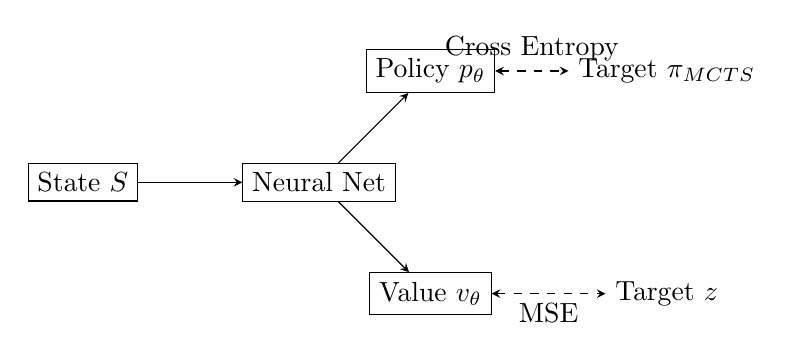
\begin{tikzpicture}[>=stealth, node distance=2cm]
  \node[draw] (state) {State $S$};
  \node[draw, right of=state, xshift=1cm] (nn) {Neural Net};
  \node[draw, above right of=nn] (pol) {Policy $p_\theta$};
  \node[draw, below right of=nn] (val) {Value $v_\theta$};

  \node[right of=pol, xshift=1cm] (target_p) {Target $\pi_{MCTS}$};
  \node[right of=val, xshift=1cm] (target_v) {Target $z$};

  \draw[->] (state) -- (nn);
  \draw[->] (nn) -- (pol);
  \draw[->] (nn) -- (val);

  \draw[dashed, <->] (pol) -- node[above] {Cross Entropy} (target_p);
  \draw[dashed, <->] (val) -- node[below] {MSE} (target_v);
\end{tikzpicture}
\end{center}

\textbf{1. Given:}
\begin{itemize}
    \item Targets: $\pi = [0.2, 0.8], z=1$.
    \item Predictions: $p = [0.4, 0.6], v=0.1$.
\end{itemize}

\textbf{2. Formula:}
$$ L = (z - v)^2 - \sum \pi_i \ln p_i $$

\textbf{3. Explanation:}
AlphaZero minimizes error in value prediction (MSE) and difference between neural policy and MCTS policy (Cross Entropy).

\textbf{4. Calculation:}
\textit{Value Loss:}
$$ (1 - 0.1)^2 = 0.9^2 = 0.81 $$

\textit{Policy Loss:}
$$ -[ 0.2 \ln(0.4) + 0.8 \ln(0.6) ] $$
$$ \ln(0.4) \approx -0.916 $$
$$ \ln(0.6) \approx -0.511 $$
$$ -[ 0.2(-0.916) + 0.8(-0.511) ] $$
$$ -[ -0.183 - 0.409 ] = -[-0.592] = 0.592 $$

\textit{Total:}
$$ 0.81 + 0.592 = 1.402 $$

\textbf{Final Answer:}
$L = 1.402$
\end{solutionbox}
\newpage

% Problem 4.6
\begin{problembox}{4.6: MuZero Hidden State Dynamics}
MuZero uses a dynamics function $g(s,a)$ to predict the next hidden state.
Hidden state $h_t = [0.5, 0.5]$.
Action $a_t$ is encoded as $[1, 0]$.
Dynamics function is a simple matrix multiplication $W[h; a]$.
$W = [[1, 0, 0, 0], [0, 1, 0, 0]]$ (Identity for h part).
Calculate $h_{t+1}$.
\end{problembox}

\begin{guidebox}
Concatenate $h$ and $a$, multiply by $W$.
\end{guidebox}

\begin{solutionbox}
\textbf{1. Given:}
\begin{itemize}
    \item $h_t = [0.5, 0.5]^T$.
    \item $a_t = [1, 0]^T$.
    \item $W$ is $2 \times 4$.
\end{itemize}

\textbf{2. Formula:}
$$ h_{t+1} = W \times \text{concat}(h_t, a_t) $$

\textbf{3. Calculation:}
Concat Vector $x = [0.5, 0.5, 1, 0]^T$.

Row 1 of W: $[1, 0, 0, 0]$.
$$ 1(0.5) + 0 + 0 + 0 = 0.5 $$

Row 2 of W: $[0, 1, 0, 0]$.
$$ 0 + 1(0.5) + 0 + 0 = 0.5 $$

\textbf{Final Answer:}
$h_{t+1} = [0.5, 0.5]$
\end{solutionbox}
\newpage

% Problem 4.7
\begin{problembox}{4.7: Dyna-Q Planning}
In Dyna-Q, the agent performs $N$ planning steps for every 1 real step.
Real step: $(S, A, R, S')$. Update $Q(S,A)$.
Planning: Select random observed $(S,A)$, get predicted $(R, S')$, update $Q$.
If $N=5$, how many total Q-updates occur in one loop?
\end{problembox}

\begin{guidebox}
Direct + Planned.
\end{guidebox}

\begin{solutionbox}
\textbf{1. Given:}
\begin{itemize}
    \item Planning steps $N=5$.
    \item Real steps per loop = 1.
\end{itemize}

\textbf{2. Formula:}
Total Updates = Real Update + Planning Updates.

\textbf{3. Explanation:}
Dyna-Q learns from real experience (Direct RL) and simulated experience from a learned model (Planning).

\textbf{4. Calculation:}
$$ 1 + 5 = 6 $$

\textbf{Final Answer:}
6 updates.
\end{solutionbox}
\newpage

% Problem 4.8
\begin{problembox}{4.8: Model Error Calculation}
Learned Model $M(s,a) \rightarrow (r, s')$.
True Environment $E(s,a) \rightarrow (10, s_{true})$.
Model predicts $r = 8$.
Calculate the prediction error for reward.
\end{problembox}

\begin{guidebox}
$|r_{true} - r_{pred}|$.
\end{guidebox}

\begin{solutionbox}
\textbf{1. Given:}
\begin{itemize}
    \item True Reward $R=10$.
    \item Predicted Reward $\hat{R}=8$.
\end{itemize}

\textbf{2. Formula:}
Absolute Error: $|R - \hat{R}|$.

\textbf{3. Calculation:}
$$ |10 - 8| = 2 $$

\textbf{Final Answer:}
Error = 2
\end{solutionbox}
\newpage

% Problem 4.9
\begin{problembox}{4.9: Curiosity Driven Exploration}
Intrinsic reward $r_i$ is defined as the forward model prediction error.
State $s_t$, Action $a_t$.
True next state $\phi(s_{t+1}) = [1, 2]$.
Predicted next state $\hat{\phi}(s_{t+1}) = [1.2, 1.8]$.
Calculate $r_i = \frac{1}{2} \|\phi - \hat{\phi}\|^2$.
\end{problembox}

\begin{guidebox}
Squared Euclidean distance.
\end{guidebox}

\begin{solutionbox}
\textbf{1. Given:}
\begin{itemize}
    \item True feature $\phi = [1, 2]$.
    \item Pred feature $\hat{\phi} = [1.2, 1.8]$.
\end{itemize}

\textbf{2. Formula:}
Intrinsic Reward:
$$ r_i = \frac{1}{2} \sum (\phi_k - \hat{\phi}_k)^2 $$

\textbf{3. Explanation:}
The agent gets a bonus reward for encountering states it cannot predict well (high "surprise").

\textbf{4. Calculation:}
Differences:
$$ d_1 = 1 - 1.2 = -0.2 $$
$$ d_2 = 2 - 1.8 = 0.2 $$

Squared Differences:
$$ (-0.2)^2 = 0.04 $$
$$ (0.2)^2 = 0.04 $$

Sum:
$$ 0.04 + 0.04 = 0.08 $$

Halve:
$$ 0.5 \times 0.08 = 0.04 $$

\textbf{Final Answer:}
$r_i = 0.04$
\end{solutionbox}
\newpage

% Problem 4.10
\begin{problembox}{4.10: Branching Factor in Search}
A game has an average branching factor $b=3$.
We search to depth $d=4$.
How many leaf nodes are there in the full tree?
\end{problembox}

\begin{guidebox}
$N = b^d$.
\end{guidebox}

\begin{solutionbox}
\textbf{1. Given:}
\begin{itemize}
    \item Branching factor $b=3$.
    \item Depth $d=4$.
\end{itemize}

\textbf{2. Formula:}
Leaf Nodes $N \approx b^d$.

\textbf{3. Explanation:}
At each level, the number of nodes multiplies by $b$.

\textbf{4. Calculation:}
$$ 3^4 = 3 \times 3 \times 3 \times 3 $$
$$ = 9 \times 9 = 81 $$

\textbf{Final Answer:}
81 nodes.
\end{solutionbox}
\newpage

% Problem 4.11
\begin{problembox}{4.11: Rollout Policy vs Tree Policy}
In MCTS, the Tree Policy uses UCT to select actions within the tree.
The Rollout Policy uses random actions to simulate the rest of the game.
If the Rollout Policy has a bias (e.g., favors capturing pieces), how does this affect the value estimate?
\end{problembox}

\begin{guidebox}
Biased rollouts lead to biased value estimates.
\end{guidebox}

\begin{solutionbox}
\textbf{Detailed Explanation:}
\begin{itemize}
    \item \textbf{Given:} A biased rollout policy (favors aggression).
    \item \textbf{Logic:} MCTS estimates $Q(s,a)$ by averaging the results of rollouts. If the rollout policy plays unrealistically (e.g., always attacking, never defending), the outcome of the simulation $G$ will not reflect optimal play.
    \item \textbf{Result:} A state might look like a "win" because the biased rollout captured a piece, even if a rational opponent would have checkmated the agent immediately after.
    \item \textbf{Conclusion:} The value estimate converges to the value of the game *under the specific rollout policy*, which may be significantly different from the true Minimax value.
\end{itemize}
\end{solutionbox}
\newpage

% Problem 4.12
\begin{problembox}{4.12: AlphaGo Search Probabilities}
The visit counts at the root are $N(a_1)=90, N(a_2)=10$.
Temperature parameter $\tau = 1$.
Calculate the policy $\pi(a|s)$ resulting from the search.
\end{problembox}

\begin{guidebox}
$\pi(a|s) = N(a)^{1/\tau} / \sum N(b)^{1/\tau}$.
\end{guidebox}

\begin{solutionbox}
\textbf{1. Given:}
\begin{itemize}
    \item $N(a_1)=90, N(a_2)=10$.
    \item $\tau = 1$.
\end{itemize}

\textbf{2. Formula:}
$$ \pi(a) \propto N(a)^{1/\tau} $$
Since $\tau=1$, this is just proportional to counts.

\textbf{3. Explanation:}
AlphaGo derives its policy vector directly from the visit counts of the MCTS.

\textbf{4. Calculation:}
Total Counts: $90 + 10 = 100$.
Probability 1:
$$ \pi(a_1) = \frac{90}{100} = 0.9 $$
Probability 2:
$$ \pi(a_2) = \frac{10}{100} = 0.1 $$

\textbf{Final Answer:}
$\pi = [0.9, 0.1]$
\end{solutionbox}

\end{document}
